\begin{frame}{String Method in Collective Variables (SMCV)}
\begin{tikzpicture}
\pcuad{\textwidth}{\textheight}
\path(nw) 
    ++(0,-0.5) node(title1)[anchor=north west,text width=\textwidth]{
        \nohyphens{A convergent approach to find \textcolor{red!80!black}{minimum free-energy (reversible) pathways} in feature space represented by sequences of system {\bf images}}
    }
    ++(0,-0.1\bbh) node(graphic1)[anchor=north west]{
        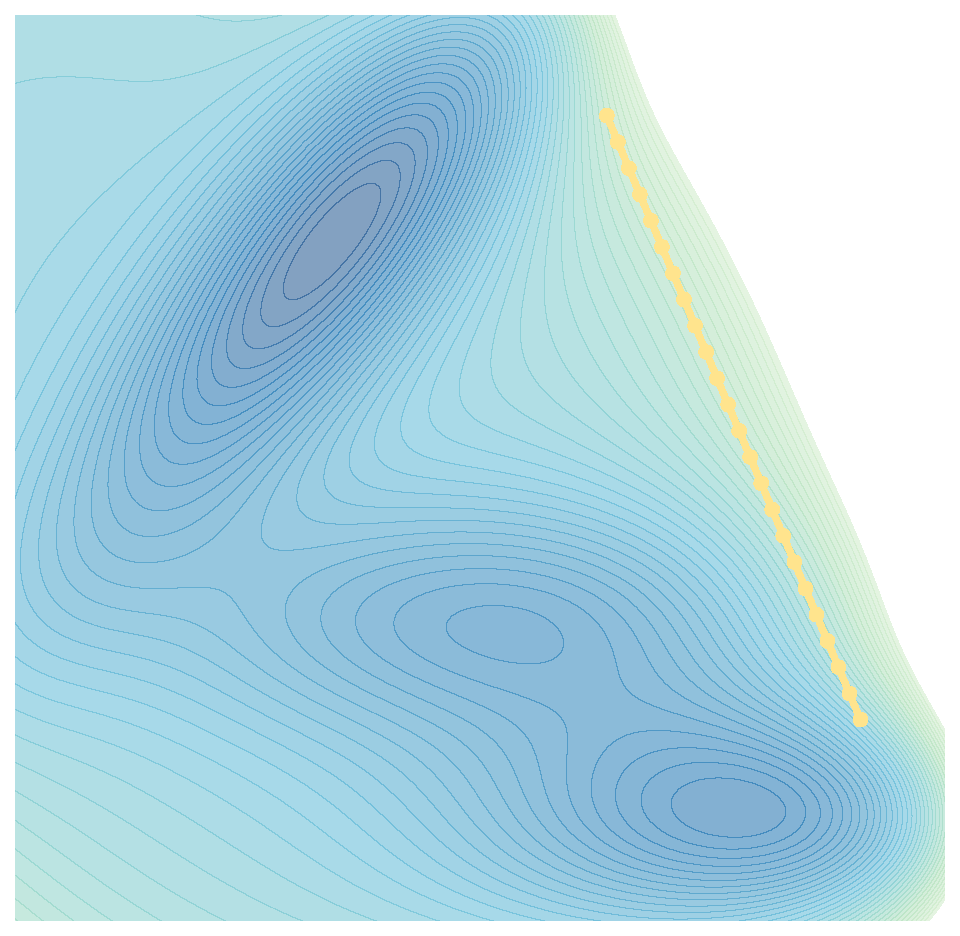
\includegraphics[width=0.25\textwidth]{sm0.pdf}
    }
    ++(0.25\bbw,0) node(graphic2)[anchor=north west]{
        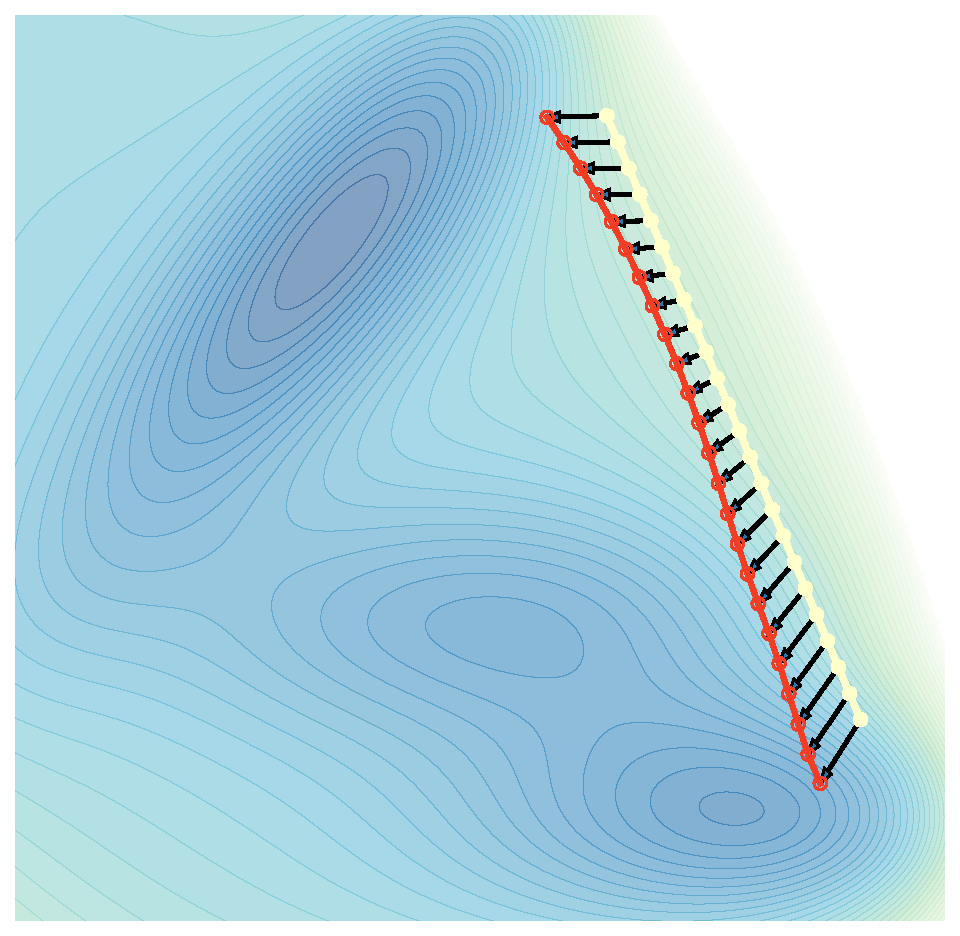
\includegraphics[width=0.25\textwidth]{sm1.pdf}
    }
    ++(0.25\bbw,0) node(graphic3)[anchor=north west]{
        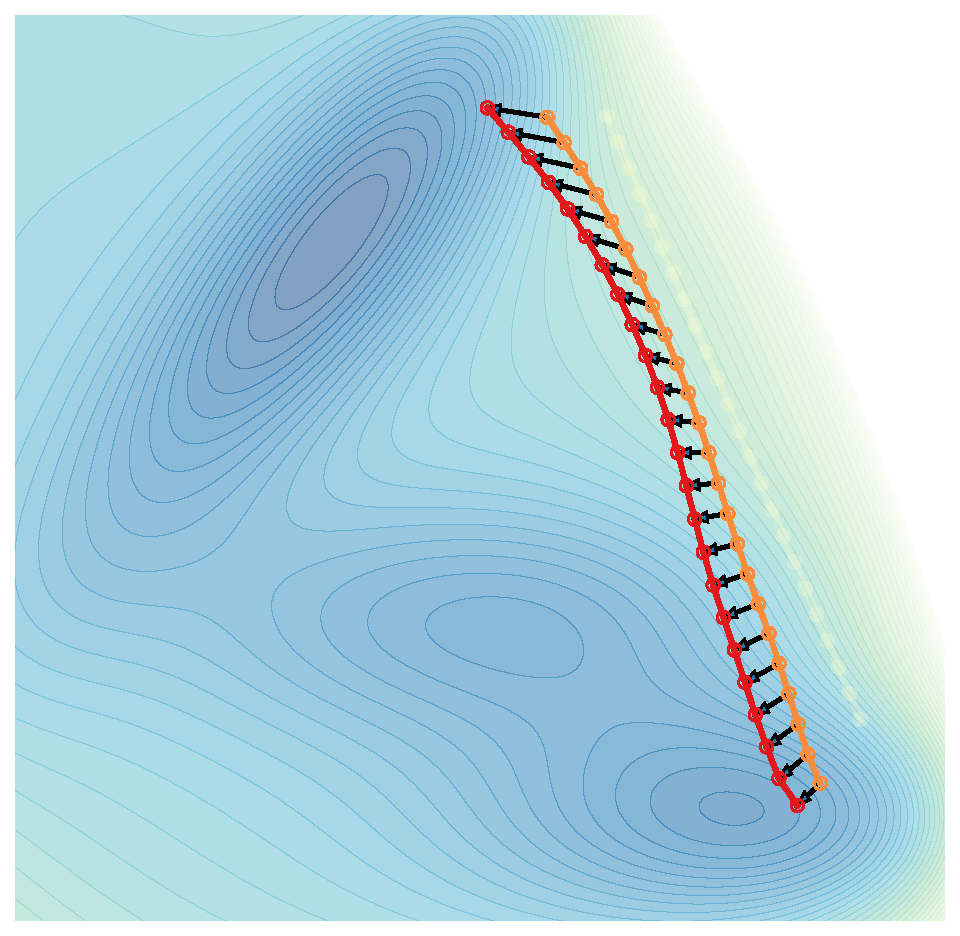
\includegraphics[width=0.25\textwidth]{sm2.pdf}
    }
    ++(0.25\bbw,0) node(graphic4)[anchor=north west]{
        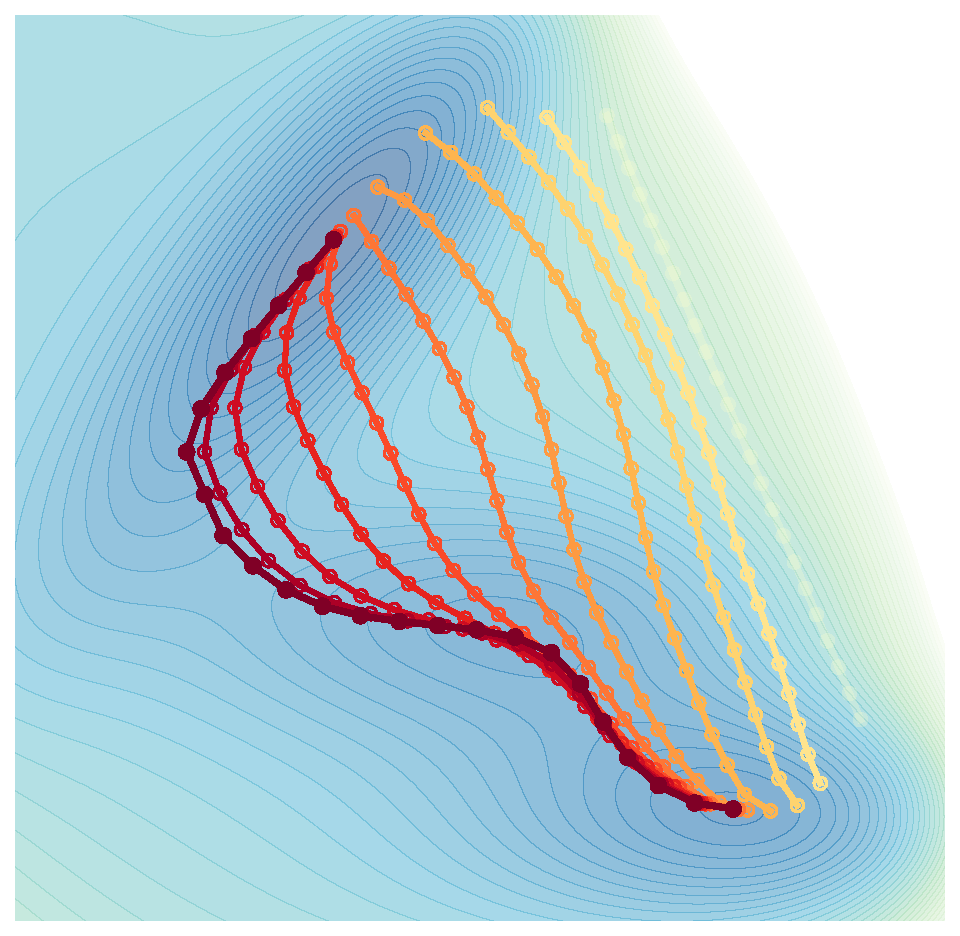
\includegraphics[width=0.25\textwidth]{sm3.pdf}    
    };
\path(cp) 
    ++(0,0) node(label1)[anchor=north]{
        Initial image positions: 
        $\left\{\zb\right\}(0)\equiv\left\{\zb_1(0),\zb_2(0),\dots,\zb_M(0)\right\}$
    }
    ++(0,-0.06\bbh) node(label2)[anchor=north]{
        Image updates: 
        $\left\{\zb\right\}(t+\Delta t)=\left\{\zb\right\}(t)-\Delta t\frac{\displaystyle\partial F}{\displaystyle\partial\left\{\zb\right\}}+\mbox{reparam.}$
    }
    ++(0,-0.12\bbh) node(label3)[anchor=north]{
        Mean forces on image 
        $i$: $-\frac{\displaystyle\partial F}{\displaystyle\partial\zb_i}=\langle\kappa\left[\thetab_i(\xb_i)-\zb_i\right]\rangle_{\zb_i}$
    }
    ++(0,-0.12\bbh) node(label4)[anchor=north]{
        found by restrained MD: 
        $\displaystyle\langle\kappa\left[\thetab_i(\xb_i)-\zb_i\right]\rangle_{\zb_i}=\frac{1}{N_{s}}\sum_{j=1}^{N_s}\kappa\left\{\thetab_i[\xb_i(t_j^{MD})]-\zb_i\right\}$
    };
\end{tikzpicture}
\end{frame}
